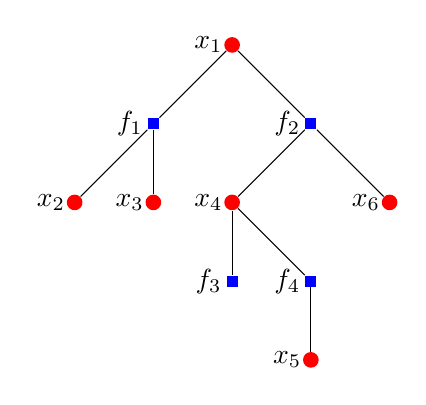
\begin{tikzpicture}[scale=1]
 \tikzstyle{cnode}=[rectangle, inner sep = 2pt, fill]
 \tikzstyle{vnode}=[circle, inner sep = 2pt, fill]
% \draw[color=red] (0,-2) node[vnode] (x2) {}; 
% \draw (-0.7, -2) node{$x_2$};
\draw [color=red](2,-2) node[vnode] (x1) {};
\draw (1.7, -2) node{$x_1$};
\draw [color=red](0,-4) node[vnode] (x2) {};
\draw (-0.3, -4) node{$x_2$};
\draw[color=red] (1,-4) node[vnode] (x3) {};
\draw (0.7, -4) node{$x_3$};
\draw[color=red] (2,-4) node[vnode] (x4) {};
\draw (1.7, -4) node{$x_4$};
\draw[color=blue] (2,-5) node[cnode] (f3) {};
\draw (1.7, -5) node{$f_3$};
\draw[color=blue] (3,-5) node[cnode] (f4) {};
\draw (2.7, -5) node{$f_4$};
\draw[color=red] (4,-4) node[vnode] (x6) {};
\draw (3.7, -4 ) node{$x_6$};
\draw[color=red] (3,-6) node[vnode] (x5) {};
\draw (2.7, -6) node{$x_5$};
\draw[color=blue] (1,-3) node[cnode] (f1) {};
\draw (0.7, -3) node{$f_1$};
\draw[color=blue] (3,-3) node[cnode] (f2) {};
\draw (2.7, -3) node{$f_2$};
\draw (x1) -- (f1);
\draw (x1) -- (f2);
\draw (f1) -- (x2);
\draw (f1) -- (x3);
\draw (f2) -- (x4);
\draw (f2) -- (x6);
\draw (x4) -- (f3);
\draw (f4) -- (x5);
\draw (x4) -- (f4);
\end{tikzpicture}